\documentclass{beamer}

\usepackage[english]{babel}
\usepackage[utf8]{inputenc}
\usepackage[T1]{fontenc}
\usepackage{lmodern}
\usepackage{graphicx}
\usepackage{hyperref}
\usepackage{pdfpages}
\hypersetup{colorlinks=true,urlcolor=blue,linkcolor=white}

						 
\usetheme{Warsaw}


\begin{document}

\title{UML, Une introduction  }%\LaTeX{}
\subtitle{Présentation}
\author{\href{mailto:abdoulaye.diallo@etud.univ-montp2.fr}{Abdoulaye DIALLO}\\
				%abdoulaye.diallo@etud.univ-montp2.fr\\
		\href{mailto:redoine.el-ouasti@etud.univ-montp2.fr}{Redoine El OUASTI}\\
				%redoine.el-ouasti@etud.univ-montp2.fr
				}
				
\date{\today}
\institute{abdoulaye.diallo@etud.univ-montp2.fr\\redoine.el-ouasti@etud.univ-montp2.fr\\
			\textbf{Université Montpellier II}}
\maketitle

\begin{frame}{Sommaire}
\section{Plan}
	\begin{enumerate}
		\item Introduction
			\begin{itemize}
			\item UML, C'est quoi?
			\item Un peu d'histoire
			\item Pourquoi modéliser?
			\end{itemize}
		\item Les diagrammes
		\begin{itemize}
			\setbeamertemplate{itemize item}[triangle]
			\item Diagrammes statiques (UML Structure)  
			\begin{itemize}
			
				\item diagramme de classes (Class diagram) 
				\item diagramme d'objets (Object diagram) 
				%\item diagramme de composants (Component diagram) 
				%\item diagramme de déploiement (Deployment diagram) 
				%\item diagramme de paquetages (Package diagram) 
				%\item diagramme de structures composites (Composite structure diagram) 
			\end{itemize}
			\setbeamertemplate{itemize item}[triangle]
			\item Diagrammes dynamiques (UML Behavior) 
			\begin{itemize}
			\setbeamertemplate{itemize item}[triangle]
				\item diagramme de cas d'utilisation (Use case diagram) 
				\item diagramme d'états-transitions (State machine diagram) 				
				\item diagramme d'activités (Activity diagram) 
				\item diagramme de séquence (Sequence diagram) 
				%\item diagramme de communication (Communication diagram) 	
			\end{itemize}
		\end{itemize}
		\item Conclusion
	\end{enumerate}
\end{frame}  

\section{Introduction}
\subsection{UML, c'est quoi ?}

\begin{frame}{UML, C'est quoi?}

	\begin{definition} % Définition
		UML ( Unified Modeling Language), ou Langage de modélisation unifié, est un langage de 		modélisation graphique à base de pictogrammes. 
	\end{definition}

	Comme n’importe quel type de projet, un projet informatique nécessite une phase d’\textbf{analyse}, suivi d’une étape de \textbf{conception}, d'où le rôle d'UML.
	\setbeameroption{show notes}
			\note{Phase d'analyse: bien comprendre et à décrire de façon précise les besoins des utilisateurs ou des clients.} 
			\setbeameroption{show notes}
		
	
\end{frame}  
%http://laurent-audibert.developpez.com/Cours-UML/?page=introduction-modelisation-objet#L1-4-3-a
%http://laurent-piechocki.developpez.com/uml/tutoriel/lp/cours/#LII-D-4
\subsection{Pourquoi modéliser}
\begin{frame}{Pourquoi modéliser?}
%\section{Introduction}


	\begin{definition} Modéliser, c’est décrire de manière visuelle et graphique les besoins et, les solutions fonctionnelles et techniques de votre projet logiciel.
	\end{definition}
	L’UML est avant tout un support de communication performant, qui facilite la représentation et la compréhension de solutions objet. L’UML est bien plus qu'un simple outil qui permet de dessiner des représentations mentales de projet... Il permet de parler un langage commun, normalisé mais accessible pour tous car il s’agit d’une représentation visuel.

\end{frame}

\subsection{Un peu d'histoire}
\begin{frame}{Un peu d'histoire}
%\section{Introduction}
	
	\begin{block}{Naissance} % Bloc normal
		UML est né de la fusion des trois méthodes qui ont le plus influencé la modélisation objet au milieu des années 90 : OMT, Booch et OOSE. Principalement issu des travaux de Grady Booch, James Rumbaugh et Ivar Jacobson. 
	\end{block}
	Fin 1997, UML est devenu une norme OMG (Object Management Group).\\
	%organisme créé en 1989 à l'initiative de grandes sociétés (HP, American Airlines, Philips...).\\
	UML 1.1 sorti en 1997; 4 révisions du standard (de l’UML1.1 à l’UML1.5 en 2003). Les dernières améliorations (en cours de validation en 2003) étant conséquentes, l’UML passe à une nouvelle version : l’UML 2.0\\
	 La dernière version diffusée par l'OMG est UML 2.4.1, disponible depuis août 2011.

	\note{En l'espace d'une poignée d'années, l’UML est devenu un standard incontournable à tel point qu’aujourd’hui, utiliser les technologies objet sans l’UML relève désormais de l'hérésie.}


\end{frame}

\section{Les Diagrammes}
\begin{frame}
	
	\note{Ces diagrammes, d'une utilité variable selon les cas, ne sont pas nécessairement tous produits à l'occasion d'une modélisation. Les plus utiles pour la maîtrise d'ouvrage sont les diagrammes d'activités, de cas d'utilisation, de classes, d'objets, de séquence et d'états-transitions.}
	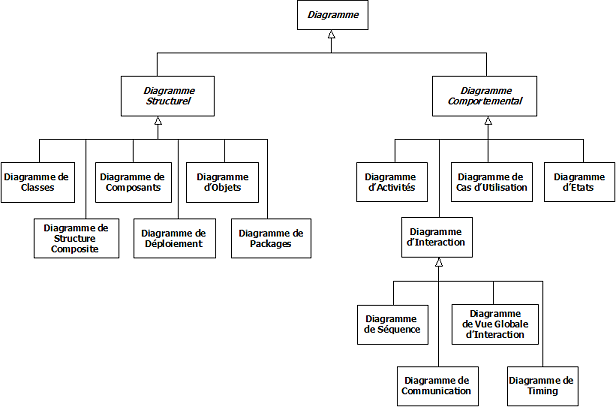
\includegraphics[width=11cm,height=7cm]{images/diag.png}


\end{frame}

\subsection{Diagramme de classes}
\begin{frame}
	%\section{Les Diagrammes}
	
	\begin{block}{Diagramme de classes}
		Représente l'architecture conceptuelle du système.\\
		considéré comme le plus important de la modélisation orientée objet, il est le seul 		obligatoire lors d'une telle modélisation.
	\end{block}
		
	Caractéristiques:
	%\pause	
	\begin{itemize}
		\item Encapsulation, visibilité
		\item attributs et méthodes 
		\item Relations entre classes
			\begin{itemize}
				\item association (multiplicité)
				\item Agrégation et composition
				\item Héritage
			\end{itemize}
	\end{itemize}
	

\end{frame}

\begin{frame}
	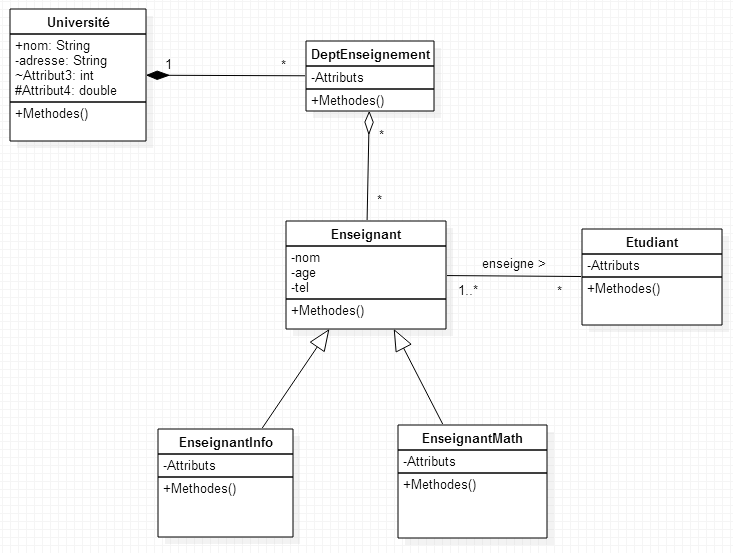
\includegraphics[width=11cm,height=8cm]{images/diagClasses.png}
\end{frame}

\subsection{Diagramme d’objet}
\begin{frame}
	\begin{block}{Diagramme d'objets}
	représente des objets (i.e. instances de classes) et leurs liens (i.e. instances de relations) pour donner une vue figée de l'état d'un système à un instant donné.
	
	\end{block}
	Il est, par exemple, utilisé pour vérifier l'adéquation d'un diagramme de classes à différents cas possibles.
\end{frame}

\begin{frame}
	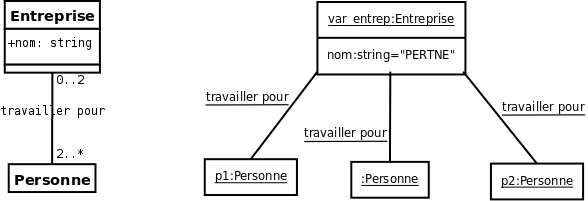
\includegraphics[width=11cm,height=6cm]{images/diagObjet}
\end{frame}

%\section{Diagrammes dynamiques}
\subsection{Diagramme de cas d'utilisation}
\begin{frame}
	\begin{block}{Diagramme de cas d'utilisation}
	Un diagramme de cas d'utilisation capture le comportement d'un système, d'un sous-			système, d'une classe ou d'un composant tel qu'un utilisateur extérieur le voit.
	\end{block}
	\note{Il ne faut pas négliger cette première étape pour produire un logiciel conforme aux attentes des utilisateurs. Pour élaborer les cas d'utilisation, il faut se fonder sur des entretiens avec les utilisateurs.}
	Éléments des diagrammes de cas d'utilisation:
	\begin{itemize}
	\item Acteur
	\item Cas d'utilisation
	\item Relation entre cas d'utilisation
	\end{itemize}
	

\end{frame}

\begin{frame}

	\begin{figure}
		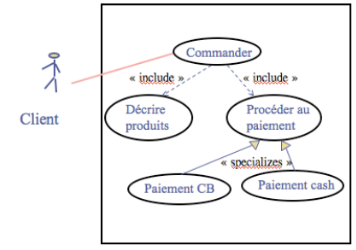
\includegraphics[width=6cm,height=4cm]{images/diagUseCase}\hfill
		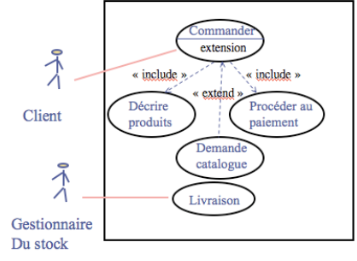
\includegraphics[width=6cm,height=4cm]{images/diagUseCase2}
		\caption{Titre commun}
	\end{figure}
		
\end{frame}

\subsection{Diagramme d'états-transitions}
\begin{frame}
	\begin{block}{Diagramme d'états-transitions (ou machine à état)}
	Permettent de décrire les changements d'états d'un objet ou d'un composant,en réponse aux interactions avec d'autres objets/composants ou avec des acteurs.
	%Représente la façon dont évoluent (i.e. cycle de vie) les objets appartenant à une même 	classe.
	\end{block}
	La vision globale du système n'apparaît pas sur ce type de diagrammes puisqu'ils ne 		s'intéressent qu'à un seul élément du système indépendamment de son environnement.\\
	Caractéristiques:
	\begin{itemize}
		\item Notion d'états (initial et final)
		\item Notion d'événement
		\item Transition
		\item États composites

	\end{itemize}

\end{frame}

\begin{frame}
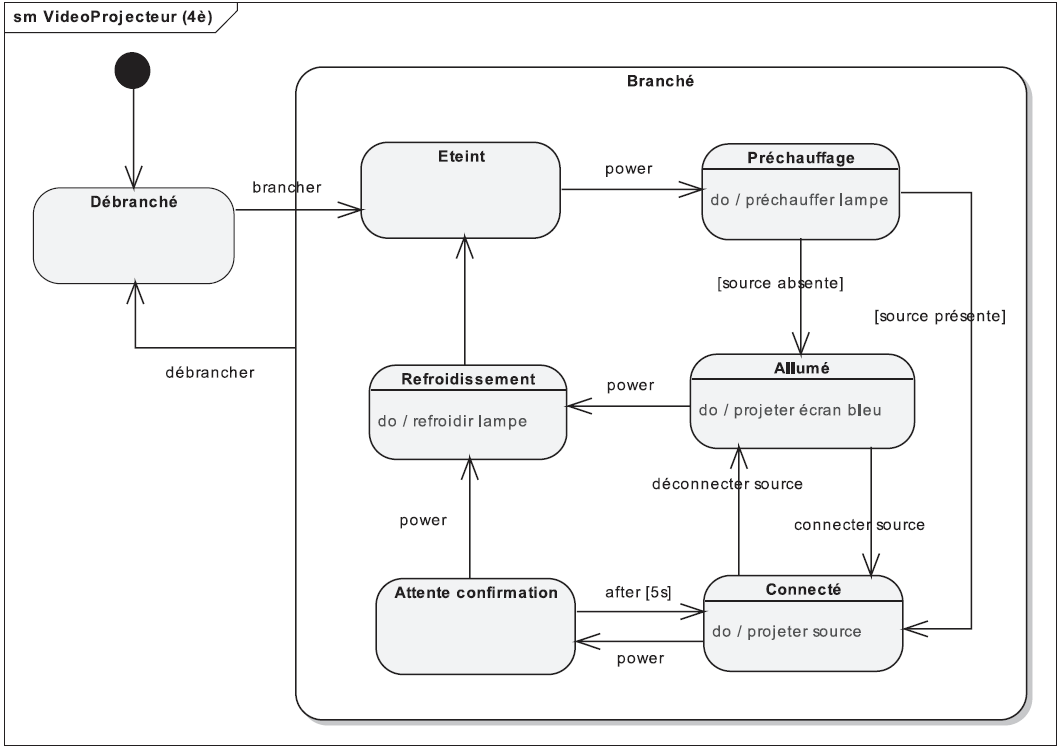
\includegraphics[width=12cm,height=8cm]{images/diagEtatTransition3}

\end{frame}

\subsection{Diagramme d'activité}
\begin{frame}
	\begin{block}{Diagramme d'activité}
	Ils permettent ainsi de représenter graphiquement le comportement d'une méthode ou le déroulement d'un cas d'utilisation.
	\end{block}
	Une activité représente une exécution d' un mécanisme, un déroulement d'étapes séquentielles.\\Le passage d'une activité à une autre est matérialisé par une transition

Caractéristiques
	 
	\begin{itemize}
	\item Noeuds d'activités: \\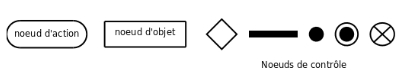
\includegraphics[width=7cm,height=2cm]{images/ndectrl}
		%Noeud initial, final(fin activité, fin de flot),de decision et de fusion,de bifurcation et d'union
	\item Transition, couloir d'activité

	\end{itemize}


	
\end{frame}	
\begin{frame}{exemple}
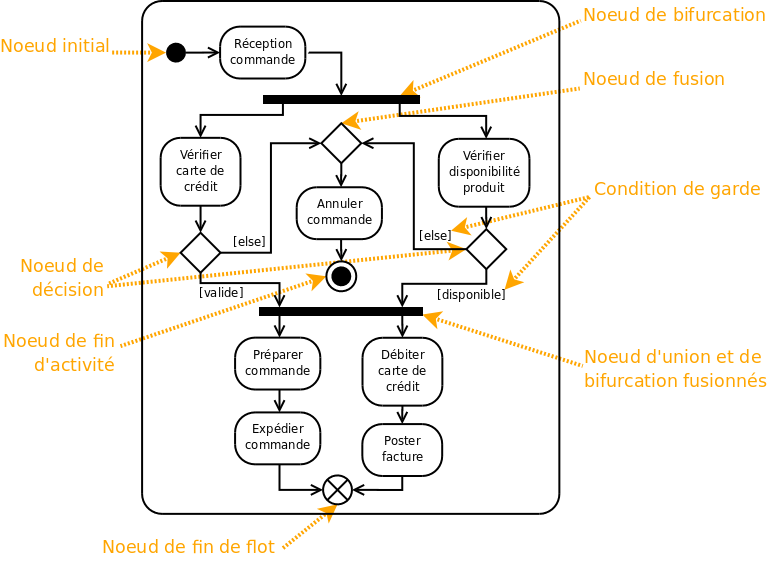
\includegraphics[width=11cm,height=6cm]{images/act3}
\end{frame}


\begin{frame}
\begin{alertblock}{Attention}
Les diagrammes d'activités sont relativement proches des diagrammes d'états-transitions dans leur présentation, mais leur interprétation est sensiblement différente;\\
machine à états décrit l’Enchaînement de tous les états d'objet(état, événement, transition). %\\En outre on est quasiment au niveau algorithme ...
\end{alertblock}	

	
\end{frame}


\subsection{Diagramme de Séquence}
\begin{frame}
	\begin{block}{Diagramme de Séquence}
		représente la succession chronologique des opérations réalisées par un acteur.\\
	Il indique les objets que l'acteur va manipuler et les opérations qui font passer d'un 		objet à l'autre
	\end{block}
	Caractéristiques
	\begin{itemize}
	\item ligne de vie (le temps s'écoule de haut en bas)
	\item messages : envoi d'un signal, opération, instanciation
	\end{itemize}
	
	


\end{frame}

\begin{frame}

\begin{columns}
\begin{column}{4cm}
	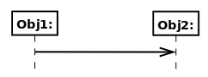
\includegraphics[width=4cm,height=2cm]{images/seq5}\\
	\textit{messages asynchrones}\\
	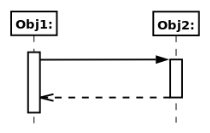
\includegraphics[width=4cm,height=2cm]{images/seq7}\\
	\textit{Messages synchrones}

\end{column}

\begin{column}{8cm}
	        
	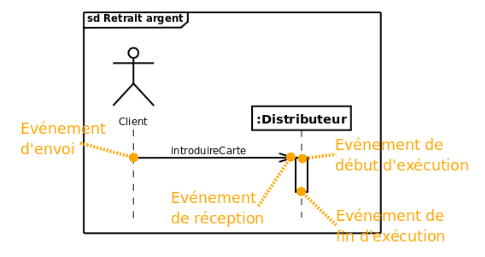
\includegraphics[width=8cm,height=6cm]{images/seq4}
	\center{\textit{Événement et messages}}
\end{column}
\end{columns}

\end{frame}


\begin{frame}
	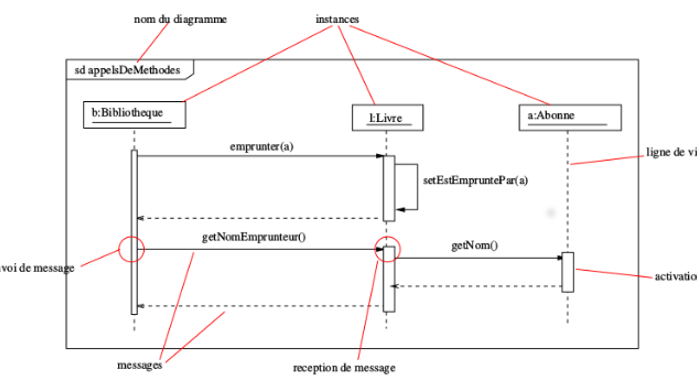
\includegraphics[width=12cm,height=8cm]{images/diagSeq2}

\end{frame}

\section{Conclusion}
\begin{frame}{Conclusion}
 UML est un langage formel et normalisé.\\
Il permet le gain de précision (et aussi de temps), encourage l'utilisation d'outils et constitue à cet effet un gage de stabilité. UML est un support de communication performant.\\
Il cadre l'analyse et facilite la compréhension de représentations abstraites complexes. Son caractère polyvalent et sa souplesse en font un langage universel.

\end{frame}


\begin{frame}
	
\includegraphics[width=8cm,height=5cm]{images/merci}
\end{frame}
	
\end{document}


